\chapter{The back-and-forth methodの実装} 
\label{ch:al_baf}
この章では\ref{ch:background}章で説明した数学的概念を離散化したアルゴリズムについて説明する。
\section{最適輸送の実装}
\label{sect:algorithm}

\subsection{Algorithm: 凸包}
\label{sect:al_convex_hull}
関数 \( f : \mathbb{R}^n \to \mathbb{R} \) の凸包conv $f$のについて考える。
conv $f$は$f$よりも大きくない最大の凸関数であり、
\[
    conv f = \sup_g \{ g \le f | g \text{ is convex function}\}
\]
と表すことができた。

上記を踏まえ、凸包のアルゴリズムAlgorithm\ref{al:convex hull algorithm}に示す。



\begin{algorithm}[tb]
    \caption{convex hull algorithm}
    \label{al:convex hull algorithm}
    \begin{algorithmic}[1]
        \State \textbf{Input:} array $x, y$ (coordinates of function $f$)
        \State $l = \{(0, -\infty)\}$ 
        \For {i, (nx, ny) in enumerate(zip(x(1:),y(1:)))}
            \While{True}
                \State $pi, pv \gets l(-1)$
                \State $v = \frac{ny - y(pi)} {nx - x(pi)} $
                \If{$v \le pv$}
                    \State $l \gets l(:-1)$
                \Else
                    \State $l \gets l \, \cup \, (i+1, v)$
                    \State \textbf{break}
                \EndIf
            \EndWhile
        \EndFor
        \State \textbf{return} $l$
    \end{algorithmic}
\end{algorithm}

凸包のアルゴリズムは以下のアイデアに基づいている:
\begin{enumerate}
    \item $l = \{(0, - \infty)\}$($x$座標の添字番号と2点によって作られる直線傾きを保存する) 
    \item 傾き更新(繰り返し)
    \begin{enumerate}
        \item 「一つ前の傾き$(pv)$」$ < $「現在の傾き$(v)$」$\Rightarrow$ $l$に$x$座標の添字番号$(i)$と傾き$(v)$を追加
        \item 「一つ前の傾き$(pv)$」$ > $「現在の傾き$(v)$」$\Rightarrow$ $l$から一つ前(配列$l$の最後の要素)の$x$座標の添字番号$(pi)$と傾き$(pv)$を消去
    \end{enumerate}
\end{enumerate}

例として、$x \in [1,5]$の関数$f$の凸包を考える。
\begin{equation*}
    f(x)=
    \begin{cases}
        x - 1 & \text{if $1 \le x \le 2$,} \\
        -3x + 7 & \text{if $2 \le x \le 3$,} \\
        3x - 11 & \text{if $3 \le x \le 4$,} \\
        -x + 5 & \text{if $4 \le x \le 5$.}
    \end{cases}
\end{equation*}
この時、凸包のアルゴリズムの流れは以下のようになる。
\begin{enumerate}
    \item 初期条件$l = [(0, -\infty)]$ (図\ref{convex_hull0})。
    \item $pv(=- \infty) < v(=1)$より、$l = [(0, -\infty), (1,1)]$ (図\ref{convex_hull1})。
    \item $pv(= 1) \ge v(=-3)$より、$l$から$(1, 1)$を消去。$l = [(0, -\infty)]$ (図\ref{convex_hull2}, \ref{convex_hull3})。
    \item $pv(=- \infty) < v(=-1)$より、$l = [(0, -\infty), (2,-1)]$ (図\ref{convex_hull4})。
    \item $pv(=- 1) < v(=3)$より、$l = [(0, -\infty), (2,-1), (3,3)]$ (図\ref{convex_hull5})。
    \item $pv(= 3) \ge v(=-1)$より、$l$から$(3, 3)$を消去。$l = [(0, -\infty), (2,-1)]$ (図\ref{convex_hull6}, \ref{convex_hull7})。
    \item $pv(=- 1) < v(=1)$より、$l = [(0, -\infty), (2,-1), (4,1)]$ (図\ref{convex_hull8})。
\end{enumerate}

\begin{figure}[htbp]
    \begin{tabular}{ccc}
      \begin{minipage}[t]{0.3\hsize}
        \centering
        \includegraphics[keepaspectratio, scale=0.3]{images/convex/convex_hull_0.png}
        \subcaption{初期状態}
        \label{convex_hull0}
      \end{minipage} &
      \begin{minipage}[t]{0.3\hsize}
        \centering
        \includegraphics[keepaspectratio, scale=0.3]{images/convex/convex_hull_1.png}
        \subcaption{$pv(=- \infty) < v(=1)$}
        \label{convex_hull1}
      \end{minipage} &
      \begin{minipage}[t]{0.3\hsize}
        \centering
        \includegraphics[keepaspectratio, scale=0.3]{images/convex/convex_hull_2.png}
        \subcaption{$pv(= 1) \ge v(=-3)$}
        \label{convex_hull2}
      \end{minipage} \\
   
      \begin{minipage}[t]{0.3\hsize}
        \centering
        \includegraphics[keepaspectratio, scale=0.3]{images/convex/convex_hull_0.png}
        \subcaption{$l$から$(1, 1)$を消去}
        \label{convex_hull3}
      \end{minipage} &
      \begin{minipage}[t]{0.3\hsize}
        \centering
        \includegraphics[keepaspectratio, scale=0.3]{images/convex/convex_hull_3.png}
        \subcaption{$pv(=- \infty) < v(=-1)$}
        \label{convex_hull4}
      \end{minipage} &
      \begin{minipage}[t]{0.3\hsize}
        \centering
        \includegraphics[keepaspectratio, scale=0.3]{images/convex/convex_hull_4.png}
        \subcaption{$pv(= -1) < v(=3)$}
        \label{convex_hull5}
      \end{minipage} \\  \begin{minipage}[t]{0.3\hsize}
        \centering
        \includegraphics[keepaspectratio, scale=0.3]{images/convex/convex_hull_5.png}
        \subcaption{$pv(= 3) \ge v(=-1)$}
        \label{convex_hull6}
      \end{minipage} &
      \begin{minipage}[t]{0.3\hsize}
        \centering
        \includegraphics[keepaspectratio, scale=0.3]{images/convex/convex_hull_3.png}
        \subcaption{$l$から$(3, 3)$を消去}
        \label{convex_hull7}
      \end{minipage} &
      \begin{minipage}[t]{0.3\hsize}
        \centering
        \includegraphics[keepaspectratio, scale=0.3]{images/convex/convex_hull_7.png}
        \subcaption{$pv(= -1) < v(=1)$}
        \label{convex_hull8}
      \end{minipage} 
    \end{tabular}
     \caption{凸包アルゴリズムの挙動(例)}
  \end{figure}


%%%%%%%%%%%%%%%%%%%%%%%%%%%%%%%%%%%%%%%%%%%%%%%%%%%%%%%%%%%%%%%%%%%%%%%%%%%%%%%%%%%%%%%%%%%%%

\subsection{Algorithm: Legender-Fenchel変換}
\label{sect:al_legendre}
Legendre-Fenchel 変換はの定義は以下である。
\begin{equation*}
    f^*(p) := sup_x\{p \cdot x - f(x) \} 
\end{equation*}
離散化したLegendre-Fenchel 変換は、凸関数のある点$(x(chi[i]), y(chi[i]))$における接線の傾き(微分)$p[j]$を求めるものである(図\ref{gra:legendre_mean})。



\begin{figure}
    \centering
    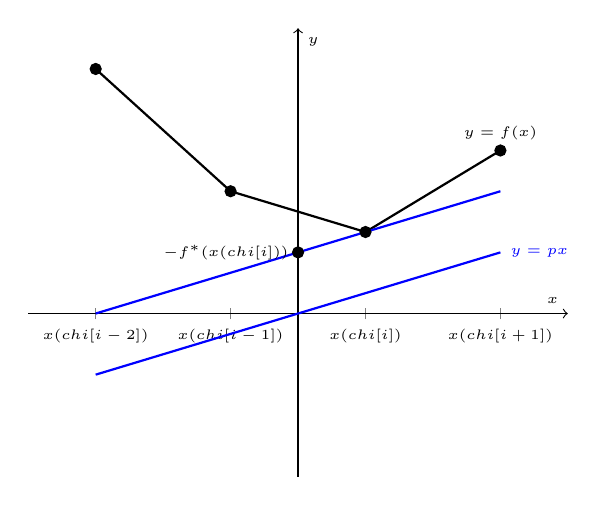
\begin{tikzpicture}
        \begin{axis}[
            xlabel={$x$},
            ylabel={$y$},
            ymin=-1, ymax=1.75,
            xmin=-2, xmax=2,
            xtick={-1.5,-0.5,0.5,1.5}, % x軸の目盛り
            xticklabels={$x(chi[i-2])$,$x(chi[i-1])$,$x(chi[i])$,$x(chi[i+1])$},
            ytick=\empty,
            axis lines=middle,
            axis line style={->},
            font=\tiny,
        ]

        % 直線の描画
        \addplot [black, thick, mark=none] coordinates {(-1.5,1.5) (-0.5,0.75)};
        \addplot [black, thick, mark=none] coordinates {(-0.5,0.75) (0.5,0.5)};
        \addplot [black, thick, mark=none] coordinates {(0.5,0.5) (1.5,1)} node[above, sloped] {$y=f(x)$};


        \addplot [blue, thick, mark=none] coordinates {(-1.5,0) (1.5,0.75)};
        \addplot [blue, thick, mark=none] coordinates {(-1.5,-0.375) (1.5,0.375)} node[right, sloped] {$y=px$};
        % 点の描画
        \addplot [only marks, mark=] coordinates {
        (-1.5,1.5)
        (-0.5,0.75)
        (0.5,0.5)
        (1.5,1)
        };
        \addplot [only marks, mark=] coordinates {(0,0.375)} node[left] {$-f^*(x(chi[i]))$};


        \end{axis}
    \end{tikzpicture}
    \caption{Legendre Fenchel変換の意味}
    \label{gra:legendre_mean}
\end{figure}




例として、$f(x) = \alpha |x|^2$とする。
このとき、
\begin{align*}
f^*(x) &= \displaystyle \sup_{p\in \Omega}{[x \cdot p - f(p)]} \quad (g(p) = x \cdot p - f(p))\\
           &=\displaystyle \sup_{p\in \Omega}{[x \cdot p - \alpha |p|^2]}\\
           &= \displaystyle \sup_{p\in \Omega}{[- \alpha(p^2 - \frac{1}{\alpha}xp)]}\\
           &= \displaystyle \sup_{p\in \Omega}{[- \alpha(p - \frac{1}{2 \alpha}x)^2 +  \frac{1}{4 \alpha}x^2]}\\
           &=  \frac{1}{4 \alpha}|x|^2 + \sup_{p\in \Omega}{[- \alpha(p - \frac{1}{2 \alpha}x)^2]}\\
           &= \frac{1}{4 \alpha}|x|^2 \qquad (\because  \text{$p = \frac{1}{2 \alpha}x$のとき,$g(p)$はsup $\Rightarrow f^*$は $p = \frac{1}{2 \alpha}x$のとき成立})\\
           &= \frac{1}{4 \alpha^2}f(x)\\
\end{align*}
よって、$\alpha = \frac{1}{2}$のとき、$f^*(x) = f(x)。$
また、$g(p)$が最大になるのは$p = \frac{1}{2 \alpha}x$のときである
$(g( \frac{1}{2 \alpha}x) = x \cdot \frac{1}{2 \alpha}x - \alpha  \frac{1}{4 \alpha^2}x^2 =  \frac{x^2}{4 \alpha} = f^*(x))$。
さらに、
$g(p) = x \cdot p - f(p)= x \cdot p - \alpha |p|^2$
であることから、
$g'(p) = 0 \Leftrightarrow x - 2 \alpha p = 0 \Leftrightarrow x - f'(p) = 0 \, (\because f'(x) = 2 \alpha x) \Leftrightarrow f'(p) = x$ 。

よって一般に、 $f(x) = \alpha |x| ^2$のとき、$f^*(p)$となる$x$は $f'(p) = x$より、ある点$p$での$f$の微分になり、 
かつ$x = f'(p) = 2\alpha p$ 。

つまり「$f^*(p)= sup_x\{p \cdot x - f(x) \} $の$x$を求めること」は 「$f'(p)$を求めること」に等しい。
よって Legendre-Fenchel transformとは,凸関数のある点$(x(chi[i]), y(chi[i])$における接線の傾き(微分)$p[j]$を求めるものである。


ここで$\alpha = \frac{1}{2}$のとき、 $f^*(x) = f(x) かつf'(p) = x = 2\alpha p = p$。

従って「$v[i]: (x(chi[i+1]), y(chi[i+1]))$と$(x(chi[i]), y(chi[i]))$を結んだ線分の傾き」$=$ 「$(x(chi[i]), y(chi[i]))$での接線の傾き(微分)」になる。
つまり、$\alpha = \frac{1}{2}$のとき、 $p$は$x$座標の分割であるので、十分小さい分割を取れば、 $p[j] = v[i]$となる$p$が必ず存在する。

特に凸関数ならば、$f^*(x)$は減少しない関数なので、$v[i]$も減少しない。
よって、$v[i] < p[j] \leq v[i+1]$となるものを見つけることができる(図\ref{gra:legendre})。この時、

\begin{center}
    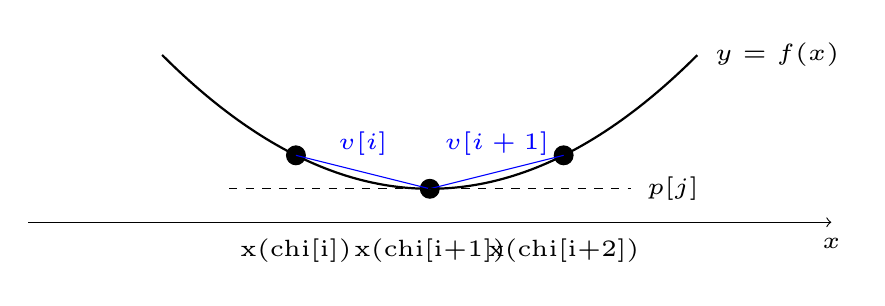
\begin{tikzpicture}[scale=1.7, transform shape]
        % グラフの描画
        \draw[->] (-3,0) -- (3,0) node[below, font=\tiny] {$x$};
        
        % 関数の描画
        \draw[black, thick, domain=-2:2, samples=100] plot (\x, {0.25*\x*\x + 0.25}) node[right, font=\tiny] {$y = f(x)$};
        
        % 点の描画
        \foreach \x/\y/\label in {-1/0.5/x(chi[i]), 0/0.25/x(chi[i+1]), 1/0.5/x(chi[i+2])}
            \filldraw (\x,\y) circle (2pt) node[below, font=\tiny] at (\x,0) {\label};
        
        % 直線の描画
        \draw[blue] (-1,0.5) -- (0,0.25) node[midway, above, font=\tiny] {$v[i]$};
        \draw[blue] (0,0.25) -- (1,0.5) node[midway, above, font=\tiny] {$v[i+1]$};
        
        % x=0での接線
        \draw[black, dashed] (-1.5,0.25) -- (1.5,0.25) node[right, sloped, font=\tiny] {$p[j]$};
        
    \end{tikzpicture}
    \captionof{figure}{Legendre Fenchel-1}
    \label{gra:legendre}
\end{center}


上記を踏まえ、Legendre-Fenchel変換のアルゴリズムAlgorithm\ref{al:legendre}に示す。

\begin{algorithm}[tb]
    \caption{Legendre-Fenchel Transform}
    \label{al:legendre}
    \begin{algorithmic}[1]
        \State \textbf{Input:} array $x, y = f(x)$ (coordinates of function $f$), $p$
        \State $chi, v \gets$ convex hull$(x, y) $
        \State $t \gets \{\}$
        \State iopt $\gets \{0,0, \dots, 0\} \quad \text{(ipot is same shape of array } x$) 
        \State $i \gets 0$
        \For {$j$, $p$ in enumerate($p$)}
            \While{$p > v(i)$}
                \State $i \gets i + 1$
            \EndWhile
            \State iopt($j$) = chi($i$)
            \State $t \gets t \cup x(\text{chi}($i$)) * p - y(\text{chi}($i$))$
        \EndFor
        \State \textbf{return} $t$, iopt
    \end{algorithmic}
\end{algorithm}

Legendre-Fenchel変換のアルゴリズムは以下のアイデアに基づいている:
\begin{enumerate}
    \item 関数$f \in \mathcal{C}$の凸包conv $f$を求める。(convex hull algorithm)
    \item 繰り返し
    \begin{enumerate}
        \item $(x(chi[i+1]), y(chi[i+1]))$と$(x(chi[i]), y(chi[i]))$を結んだ線分の傾き$v[i] \le p[j]$となる座標の添字番号$chi[i]$を見つける。
        \item $(x(chi[i]), y(chi[i]))$におけるLegendre-Fenchel変換を計算し、配列$t$に保存する。
    \end{enumerate}
\end{enumerate}
%%%%%%%%%%%%%%%%%%%%%%%%%%%%%%%%%%%%%%%%%%%%%%%%%%%%%%%%%%%%%%%%%%%%%%%%%%%%%%%%%%%%%%%%%%%%%%%%%%%%%%%%%%%%%%%%%%%%%%%%%%%%%%%%%%%%%%%%%%%

\subsection{Algorithm: $c$-変換}
\label{sect:al_c-tra}
$\varphi^c(p) = \frac{1}{\tau}\inf_x\left\{\frac{|x-p|^2}{2} - \tau\varphi(x)\right\}$について考える。
このときc変換は以下のようになる。
\begin{align*}
    \varphi^c(p) &= \frac{1}{\tau} \inf_x\left\{\frac{|x-p|^2}{2} - \tau \varphi(x)\right\}\\
              &= \frac{1}{\tau}  \left(\frac{|p|^2}{2} + \inf_x\left[- \left\{x \cdot p - \frac{|x|^2}{2} + \tau\varphi(x) \right\}\right]\right)\\
              &= \frac{1}{\tau}  \left(\frac{|p|^2}{2} - \sup_x\left[x \cdot p - \left\{\frac{|x|^2}{2} - \tau\varphi(x)\right\}\right]\right)\\
              &= \frac{1}{\tau}  \left(\frac{|p|^2}{2} - \sup_x\left\{x \cdot p - \psi(x)\right\} \qquad (\because \psi(x) = \frac{|x|^2}{2} - \tau\varphi(x))\right)\\
              &= \frac{1}{\tau}  \left(\frac{|p|^2}{2} - \psi^*(p)\right)\\
    \\
    \varphi^{cc}(q) 
              &= \frac{1}{\tau} \inf_p\left\{\frac{|p-q|^2}{2} - \tau \varphi^c(p)\right\}\\
              &= \frac{1}{\tau}\left(\frac{|q|^2}{2} + \inf_p\left[- \left\{p \cdot q - \frac{|p|^2}{2} + \tau\varphi^c(p) \right\}\right]\right)\\
              &= \frac{1}{\tau}\left(\frac{|q|^2}{2} - \sup_p\left[p \cdot q - \left\{\frac{|p|^2}{2} - \tau\varphi^c(p)\right\}\right]\right)\\
              &= \frac{1}{\tau}\left(\frac{|q|^2}{2} - \sup_p\left[p \cdot q - \left\{\frac{|p|^2}{2} - \left(\frac{|p|^2}{2} - \psi^*(p)\right)\right\}\right]\right)\\
              &= \frac{1}{\tau}\left(\frac{|q|^2}{2} - \sup_p\left[p \cdot q - \psi^*(p)\right]\right) \\
              &= \frac{1}{\tau}\left(\frac{|q|^2}{2} - \varphi^{**}(q)\right)
\end{align*}

上記を踏まえ、$c$-変換のアルゴリズムをAlgorithm\ref{al:c-transform}に示す。
アルゴリズムでは、$c$-変換を$\inf_x\left\{\frac{|x-p|^2}{2} - \varphi(x)\right\}$としている。
そのため、アルゴリズム中の$\varphi(x)$を$\tau\varphi(x)$、returnされた値$\frac{1}{2} p^2 - t$を$\frac{1}{\tau}\left(\frac{1}{2} p^2 - t\right)$とすることによって、実際の$c$-変換の値を計算している。

\begin{algorithm}[tb]
    \caption{c-transform}
    \label{al:c-transform}
    \begin{algorithmic}[1]
        \State \textbf{Input:} array $x,y = \varphi(x)$ (coordinates of function $f$), $p(=x)$
        \State $\psi(x) \gets \frac{1}{2} x^2 - \varphi(x)$
        \State $t$, index $\gets$ Legendre-Fenchel transform$(x, \psi, p)$
        \State \textbf{return} $\frac{1}{2} p^2 - t, $ index
    \end{algorithmic}
\end{algorithm}


\subsection{Algorithm: 最適輸送写像(押し出し測度)}
\label{sect:al_pushforward}
$\varphi, \psi$がどちらも$c$-凹のとき、押し出し測度$T_{\varphi \#} \mu$および$T_{\psi \#} \delta U^*(- \psi^c)$は、
\begin{equation*}
    T_{\varphi \#} \mu (y) =\mu(y - \tau \nabla \varphi(y))|\det (I - \tau D^2 \varphi(y))|
\end{equation*}
\begin{equation*}
    T_{\psi \#} \delta U^* (- \psi^c)(x) =\delta U^* (- \psi^c)(x - \tau \nabla \psi(x))|\det (I - \tau D^2 \psi(x))|
\end{equation*}
である。

押し出し測度のアルゴリズムは以下のアイデアに基づいている。
    
\begin{enumerate}
    \item 入力パラメータ:
    \begin{itemize}
        \item \texttt{mu}: セルごとの初期密度を表す配列。
        \item \texttt{phi\_c}: セルごとの位相関数を表す配列。
        \item \texttt{h}: グリッド間のセルサイズ。
    \end{itemize}

    \item 初期化:
    \begin{itemize}
        \item \texttt{t\_mu}: 結果を格納するための配列を、\texttt{mu} と同じ形状で初期化。
    \end{itemize}

    \item 各セルに対して以下を繰り返す:
    \begin{enumerate}
        \item セル番号iの近傍の3つのセル(um,u,up)における$\varphi$の$c$-変換を求める。
        \item $\varphi$の$c$-変換に対するセル$i$における勾配(dphi\_c)を中心差分法で計算する。
        \item セル \texttt{i} におけるヘッセ行列の行列式 det ($\text{det}(I - D^2\varphi_c)$) を計算する。
        \item 変形前の座標系における位置xcellの計算する。
        \item xcellに最も近いセルのインデックスtiとその次のセルtioを計算する。
        \item tiとtioにおける密度を線形補間して、xcellでの密度 mu\_inter を計算する。
        \item セルiにおける押し出し測度t\_mu[i]($T_{\varphi \#} \mu$, $T_{\psi \#} \delta U^*(- \psi^c)$)を計算する。
    \end{enumerate}

\end{enumerate}

上記を踏まえ、押し出し測度のアルゴリズムをAlgorithm \ref{alg:push_forward}に示す。
\begin{algorithm}
    \caption{Push Forward}
    \label{alg:push_forward}
    \begin{algorithmic}[1]
        \State \textbf{Input:}{$\mu, \varphi_c, h$}
        \State Initialize $t_\mu$ as a zero array of the same shape as $\mu$
        \State $n \gets \text{shape}(\varphi_c)[0]$
        \State Initialize empty lists $l_{\nabla\varphi_c}$ and $l_{\text{det}}$
        
        \For{$i$ in range($n$)}
            \State $um \gets \varphi_c[\max(i-1, 0)]$
            \State $u \gets \varphi_c[i]$
            \State $up \gets \varphi_c[\min(i+1, n-1)]$
            
            \State $\nabla\varphi_c \gets \frac{up - um}{2h}$
            \State $l_{\nabla\varphi_c}.\text{append}(\nabla\varphi_c)$
            
            \State $\text{det} \gets 1 - \frac{up - 2u + um}{h^2}$
            \State $l_{\text{det}}.\text{append}(\text{det})$
            
            \State $x_{\text{cell}} \gets i - \frac{\nabla\varphi_c}{h}$
            \State $ti \gets \text{int}(\min(\max(\lfloor x_{\text{cell}} \rfloor, 0), n - 1))$
            \State $tio \gets \min(ti + 1, n - 1)$
            
            \State $\mu_{\text{inter}} \gets \mu[ti] \left(1 - (x_{\text{cell}} - \lfloor x_{\text{cell}} \rfloor)\right) + \mu[tio] \left(x_{\text{cell}} - \lfloor x_{\text{cell}} \rfloor\right)$
            
            \State $t_\mu[i] \gets \mu_{\text{inter}} \cdot \text{det}$
        \EndFor
        
        \State \textbf{return} $t_\mu$
    \end{algorithmic}
\end{algorithm}


\section{The back-and-forth methodを用いたJKOスキームの実装}
\label{sect:algorithm}
本論文ではThe back-and-forth methodを使用して、多孔質勾配方程式
\[
    \rho_t = \frac{{\partial \rho}}{{\partial t}} = \gamma\Delta (\rho^m), \quad (\rho \geq 0, m > 1)
\]
を解く。
ただし、
\[
    \rho(t, x) := \overline{\rho}(\gamma(t+t_0), x) 
\]
とする。このとき
$
    \partial_t\rho = \gamma\partial_t\overline{\rho} 
$
より、
\begin{equation}
    \left\{ \,
    \begin{aligned}
        \rho_t - \gamma\Delta(\rho^m) & = 0 \\
        \rho(0, x) & = \overline{\rho}(\gamma t_0, x)
    \end{aligned}
    \right.
\end{equation}
と考えることができる。
初期データは
\[
    \rho(0,x) = M\delta_0(x)
\]
で与えられるとする。
ここで、\(\gamma > 0\)は拡散の速度を制御する定数、\(M > 0\)は初期総質量、\(\delta_0\)は原点を中心とする標準的なディラックのデルタ分布とする。
\(m > 1\)の場合、この方程式はエネルギー
\[
    U(\rho) = \int_\Omega \frac{\gamma}{m - 1}\rho(x)^m dx 
\]
のWasserstein勾配流となる。
領域\(R\)上で閉じた解が存在し、これはBarenblatt solutionとして知られている。
Barenblatt solutionは安定性条件を必要としないため、非常に有効な近似解を得ることができる。
Barenblatt solutionは以下のように与えられる(ただし、$(\cdot)_+ = max(\cdot, 0), \alpha = \frac{1}{m + 1}, \beta = \frac{1}{m + 1}$):
\begin{equation}
    \label{eq:barenblatt}
    \rho(t,x)= \frac{1}{t^\alpha}\left(b - \frac{m - 1}{2m}\frac{\beta |x|^2}{t^{2\beta}} \right)_+^{\frac{1}{m - 1}}
\end{equation}

ここで例として$m = 2$のとき、
\begin{equation}
    \label{eq:barenblatt:m=2}
    \rho(t,x)= \frac{1}{t^{\frac{1}{3}}}\left(b - \frac{1}{12} \frac{ |x|^2}{t^{\frac{2}{3}}} \right)_+
\end{equation}
となる。さらに、
\begin{align*}
    \rho(t, x) = 0 &\iff \frac{1}{t^{\frac{1}{3}}}\left(b - \frac{1}{12} \frac{ |x|^2}{t^{\frac{2}{3}}} \right) = 0,\\
                    &\iff b = \frac{1}{12}\frac{|x|^2}{t^{\frac{2}{3}}}, \\
                    &\iff |x|^2 = 12t^{\frac{2}{3}}b \iff x = \pm \sqrt{12t^{\frac{2}{3}}b},
\end{align*}



\begin{align*}
    \int^{+\infty}_{-\infty} \rho(t, x)dx &= 2 \int^{\sqrt{12t^{\frac{2}{3}}b}}_0 \frac{1}{t^{\frac{1}{3}}}\left(b - \frac{1}{12} \frac{|x|^2}{t^{\frac{2}{3}}}\right)dx,\\
                                            &= \frac{2}{t^{\frac{1}{3}}}\left(b r - \frac{r^3}{3 \cdot 12 t^{\frac{2}{3}}}\right) \qquad \left(\because r := \sqrt{12t^{\frac{2}{3}}b}\right),\\
                                            &= \frac{2}{t^{\frac{1}{3}}}\left(b r - \frac{12t^{\frac{2}{3}}b r}{3 \cdot 12 t^{\frac{2}{3}}}\right) = \frac{2}{t^{\frac{1}{3}}}\frac{2}{3}br,\\
                                            &= \frac{2}{t^{\frac{1}{3}}}\frac{2}{3}b \cdot 2\cdot \sqrt{3} t^{\frac{1}{3}},\\
                                            &= \frac{8}{\sqrt{3}}b^{\frac{3}{2}} =: M  \qquad \Longrightarrow b = \left(\frac{\sqrt{3}}{8} M \right)^{\frac{2}{3}}.
\end{align*}



したがって、質量が正方形の境界に達するまでの時間$t_c$まで、$\Omega = [- \frac{1}{2}, \frac{1}{2}]$の上の解と一致することがわかる。
初期条件のディラックのデルタ関数は扱いにくいため、高さ$h_0 > 0$を固定し、時間$t_0 > 0$から開始することにする。
ここで$t_0$は、$\|\rho(0, \cdot)\|_{L^\infty}= \|\overline{\rho} (\gamma t_0, \cdot)\|_{L^\infty} = h_0$となるように選ぶ。
ただし、$t_0$は以下のように求めることができる。
\begin{align*}
    \|\rho(0, \cdot)\|_{L^\infty} = \|\overline{\rho} (\gamma t_0, \cdot)\|_{L^\infty} &= \overline{\rho}(\gamma t_0, 0) = \frac{1}{(\gamma t_{0})^{\frac{1}{3}}} b\ = h_0\\
    \Longrightarrow \, t_0 = \frac{1}{\gamma}\left(\frac{b}{h_0}\right)^3
\end{align*}
さらに、Barenblatt solutionは時間$t_c$までの間にのみ有効であるため、時間$t \in [t_0, 2.0+t_0]$のみを考慮する。
このBarenblatt solutionを基準として使用して、各アルゴリズムの精度と効率をテストしていく。
解の精度は$L^1$ノルムを使用して以下のように誤差を求めることができる。
\begin{equation}
    \label{eq:error}
    \text{error} = \frac{1}{N_\tau} \sum_{n = 0}^{N_\tau} \int_\Omega |\overline{\rho}(\gamma(n \tau + t_0), x) - \overline{\rho}^{(n)}(x)|\, dx
\end{equation}
ここでnは離散的な時間ステップを示し、$\tau$は時間のステップサイズを表す。
ただし、$N_\tau = \lfloor \frac{2}{\tau} \rfloor$であり、$\overline{\rho}(n\tau + t_0, x)$はBarenblatt solutionであり、
$\overline{\rho}^{(n)}$は初期データ$\overline{\rho}^{(0)}(x) = \overline{\rho}(\gamma t_0, x) = $から始まる$n$回目のJKOスキームである。
また$\varphi^{(n+1)}$を求める際、the back-and-forth methodを使用する。
ただし$\|\delta U^*(- \varphi) - T_{\varphi \#} \mu \|_{L^1(\Omega)}$が$\varepsilon (\text{実験では}\varepsilon = 10^{-3}, 10^{-5}, 10^{-6}\text{を使用})$未満、
もしくは繰り返しが100回より多くなるまでthe back-and-forth methodを繰り返す。

アルゴリズム実装のため、各関数の値を確認しておく。
エネルギー関数は
\[
    U(\rho) := \frac{\gamma}{{m-1}} \int \rho^m \, dx, \quad \delta U(\rho) = \frac{m \gamma}{m-1} \rho^{m-1}
\]
であり、$U$のLegendre Fenchel変換$U^*$は
\[
     U^*(- \varphi) = \sup_{\rho \in P} \int \left(- \frac{\gamma}{m-1}\rho^m - \rho\varphi\right) \, dx
\]
であった。このときLemma. \ref{lem:rho_opt}より、$U^*(- \varphi)$を最大化させる$\rho_*$は
\begin{equation}
    \label{eq:m=2rho}
    \rho_*(x) = \delta U^*(- \varphi) =  \left( \frac{m-1}{m\gamma}(C - \varphi)_+ \right)^{\frac{1}{m-1}} 
\end{equation}

となる。
以上を用いて、多孔質勾配方程式$(m=2)$におけるthe back-and-forth methodの離散化したアルゴリズムをAlgorithm \ref{al:baf}に示す。

\begin{algorithm}
    \caption{Discretised the back-and-forth method}
    \label{al:baf}
    \begin{algorithmic}[1]
        \State \textbf{Input:} $\mu = \rho^{(0)} = \max\left(\frac{1}{(\gamma t_0)^{1/3}}\left(b - \frac{1}{12}\frac{x^2}{(\gamma t_0)^{2/3}}\right),0\right), \varphi_0 = \delta U(\rho^{(0)}) = \frac{m \gamma}{m-1} \left(\rho^{(0)}\right)^{m-1}$
        \While{$\text{diff} \geq \varepsilon$}
            \If{$\text{count} > 100$}
                \State \textbf{break}
            \EndIf
            \State $\rho \leftarrow \left(\frac{m-1}{m\gamma}\max(c - \varphi, 0)\right)^{1/(m-1)}$
            \State $\varphi, \psi, \text{pfwd} \leftarrow \text{ascent}(\varphi, \psi, \mu, \rho)$ (Algorithm \ref{al:ascent})
            \State $\text{diff} \leftarrow \sum \left|\rho - \text{pfwd}\right| \cdot h$
    
            \State $\psi_c, \_ \leftarrow \text{c\_transform}(x, \tau \cdot \psi, x)$ 
            \State $\psi_c \leftarrow \frac{\psi_c}{\tau}$
    
            \State $\rho \leftarrow \left(\frac{m-1}{m\gamma}\max(c - \psi_c, 0)\right)^{1/(m-1)}$
            \State $\psi, \varphi, \text{pfwd} \leftarrow \text{ascent}(\psi, \varphi, \rho, \mu)$
    
            \State $\text{count} \leftarrow \text{count} + 1$
        \EndWhile
    \end{algorithmic}
\end{algorithm}
ここで、Algorithm \ref{al:baf}の7行目ascentとはAlgorithm \ref{al:ascent}を指す。
また、Algorithm \ref{al:ascent}の8行目gauss$(\rho - \text{pfwd}, \Theta_1, \Theta_2)$ とは、
\[
    (\Theta_1 \text{Id} - \Theta_2 \Delta)u = f
\]
において、$f = \rho - \text{pfwd}$のとき$u = \text{lp}$を求めるものである。
    \begin{algorithm}
        \caption{Ascent in Algorithm \ref{al:baf}}
        \label{al:ascent}
        \begin{algorithmic}[1]
            \State \textbf{Input:} $\varphi$, $\varphi_c$, $\mu$, $\rho$
            \State $\varphi_c, \_ \leftarrow \text{c\_transform}(x, \tau \cdot \varphi, x)$ 
            \State $\varphi_c \leftarrow \frac{\varphi_c}{\tau}$
        
            \State $n\mu \leftarrow \max(\lVert\mu\rVert_\infty)$
            \State $\Theta_1 \leftarrow \frac{1}{2\gamma}$
            \State $\Theta_2 \leftarrow \tau \cdot n\mu$
        
            \State $\text{pfwd} \leftarrow \text{push\_forward}(\mu, \tau \cdot \varphi, h)$ 
            \State $lp \leftarrow \text{gauss}(\rho - \text{pfwd}, \Theta_1, \Theta_2)$ 
            \State $\varphi \leftarrow \varphi + lp$ 
            
            \State $\varphi_c, \_ \leftarrow \text{c\_transform}(x, \tau \cdot \varphi, x)$
            \State $\varphi_c \leftarrow \frac{\varphi_c}{\tau}$
    
            \State \textbf{return}  $\varphi, \varphi_c, \text{pfwd}$ 
        \end{algorithmic}
    \end{algorithm}